\section{卖方样本的价值与局限}

本案收集 38 份原始卖方 PDF，覆盖 14 个重点代码与 2 份行业报告。卖方样本的主要价值是提供可复算的 2026E/2027E 收入、净利和 EPS，以及少数明示目标价；它并不能替代公司公告确认 Atlas 950 供应关系。大多数公司报告讨论的是全球 AI 光互联、AI PCB、液冷、昇腾生态或国产超节点需求，而不是经过公司确认的 Atlas 950 订单。

\begin{exhibitbox}[重点代码卖方一致预期]
\begin{longtable}{L{1.5cm}L{2.1cm}R{1.5cm}R{1.7cm}R{1.7cm}R{1.5cm}L{3.0cm}}
\toprule
\textbf{代码} & \textbf{公司} & \textbf{样本数} & \textbf{2026E NP} & \textbf{重算 EPS} & \textbf{现价 PE} & \textbf{明示目标/缺口}\\
\midrule
\endhead
000034 & 神州数码 & 1 & 9.03 & 0.888 & 27.7x & 未披露目标价\\
000988 & 华工科技 & 2 & 23.74 & 2.361 & 49.8x & 未披露目标价\\
600183 & 生益科技 & 3 & 55.68 & 2.292 & 57.7x & 103.50 元\\
002916 & 深南电路 & 3 & 54.71 & 8.031 & 41.6x & 288.00 元\\
002463 & 沪电股份 & 6 & 57.20 & 2.972 & 43.0x & 未披露目标价\\
300476 & 胜宏科技 & 3 & 88.98 & 9.054 & 26.7x & 未披露目标价\\
002837 & 英维克 & 2 & 11.43 & 0.897 & 68.6x & 未披露目标价\\
301018 & 申菱环境 & 1 & 4.28 & 1.144 & 76.0x & 未披露目标价\\
002335 & 科华数据 & 1 & 6.95 & 0.921 & 32.3x & 未披露目标价\\
002130 & 沃尔核材 & 1 & 18.80 & 1.343 & 11.3x & 未披露目标价\\
002230 & 科大讯飞 & 2 & 12.07 & 0.503 & 81.8x & 未披露目标价\\
002025 & 航天电器 & 4 & 3.80 & 0.836 & 77.4x & 69--78 元；预测分歧大\\
\bottomrule
\end{longtable}
\sourcenote{单位：净利润亿元、EPS 元。净利润来自正权重原始 PDF；EPS 统一按 2026-07-17 市值/收盘价推导的现股本重算，避免送转股口径污染。}
\end{exhibitbox}

航天电器是卖方样本中最容易被“能力叙事”误读的公司：2026E EPS 从 0.53 到 1.10 元、2027E 从 0.62 到 2.15 元，预测区间远宽于多数硬件公司；最新 69--78 元目标区间也属于卖方对公司整体连接器/军工业务的判断，并非 Atlas 950 专属目标。拓维信息则相反，年报对华为购销和昇腾伙伴关系更直接，但 180 天内没有新鲜原始卖方预测，且 FY2025 扣非亏损、2026Q1 扣非仍亏损，因此不能用旧报告的当前价 PE 反推目标价。前者要先验证客户与毛利，后者要先验证经常性利润与新鲜预测。

\section{一致预期的三个盲点}

\textbf{第一，行业景气与平台归属经常混写。}光模块、AI PCB、液冷的全球或国内需求可以支持公司增长，但不能据此确认来自华为 Atlas 950。若将同一份广义 AI 收入同时归因于 NVIDIA、国产算力和云厂商扩产，就会发生重复计算。

\textbf{第二，盈利预测常比目标价完整。}14 个重点代码中只有生益科技、深南电路和航天电器存在明示目标价观察；其他报告只有当前价 PE 或盈利预测。本报告对缺失目标价的 Street 权重设为 0，不用报告中的当前价 PE 反推一个并不存在的券商目标。

\textbf{第三，超节点主题容易忽略现金流与毛利率。}服务器分销、项目集成、液冷总包和高端部件的收入规模与利润质量完全不同。拓维信息的高华为购销占比伴随扣非亏损，科华数据 H1 归母增速显著高于扣非增速，申菱/英维克 Q1 利润承压；这些差异比“进入生态”更能决定估值。

\section{市场共识、AStock 分歧与反身性}

市场共识倾向于把 1,024 卡实物展示视为 8,192 卡路线图和全产业链订单的领先指标，并给光互联、PCB、液冷、连接器等环节以成长溢价。AStock 的分歧是：实物展示确实降低架构可行性风险，却没有降低客户、BOM、供应商分配和公司盈利的不确定性；后四项才决定 A 股 EPS。

最强反方观点是，供应链保密和订单节奏通常领先公开披露，等待公告可能错过估值重估。我们承认这一点，因此保留能力池和关系池；但解决方案应是提高跟踪频率与设置证据触发，而不是把传闻直接写入盈利。若 2026Q4 前后出现华为/客户交付、公司平台认证或订单、收入和毛利率连续验证，AStock 的 0 信用假设将被证明过于保守并快速上调。

反身性风险也很明确：发布会提高主题关注，价格上行抬高融资和扩产能力，又吸引更多“相关”叙事；如果后续订单不出现，高估值反而放大下跌。2026-07-17 多数主题股单日大跌，说明拥挤交易对新闻和风险偏好高度敏感，但大跌不等于便宜，仍需以 2026E PE 和盈利兑现衡量。

量化桥梁是：12 个建模标的现价对应 2026E PE 为 11.3--81.8 倍，中位数 46.4 倍；若用 1.0 倍 PEG 仅作透明的预期诊断，中位价格要求约 46\%的可持续净利润增长。该要求远高于“实物展示”本身能证明的盈利内容，因为 Atlas 客户、订单、ASP、公司份额与毛利仍为空。市场锚因此只占综合目标 20\%，而不是用当前价格反证基本面合理。

\begin{exhibitbox}[逐票市场隐含预期与情绪桥]
\begin{longtable}{L{1.35cm}L{1.8cm}R{1.5cm}R{1.5cm}R{1.45cm}R{1.45cm}R{1.55cm}R{1.55cm}}
\toprule
\textbf{代码} & \textbf{公司} & \textbf{隐含增长} & \textbf{27E 增长} & \textbf{缺口} & \textbf{当日涨跌} & \textbf{5日成交额} & \textbf{现价/Base}\\
\midrule
\endhead
000034 & 神州数码 & 27.7\% & 30.7\% & -3.0ppt & -8.6\% & 17.0 & +155.9\%\\
000988 & 华工科技 & 49.8\% & 27.4\% & +22.4ppt & -10.0\% & 74.7 & +194.5\%\\
600183 & 生益科技 & 57.7\% & 43.1\% & +14.6ppt & -10.0\% & 106.5 & +265.8\%\\
002916 & 深南电路 & 41.6\% & 34.4\% & +7.2ppt & -8.2\% & 55.9 & +160.9\%\\
002463 & 沪电股份 & 43.0\% & 51.7\% & -8.7ppt & -6.5\% & 104.0 & +180.6\%\\
300476 & 胜宏科技 & 26.7\% & 73.8\% & -47.2ppt & -10.9\% & 84.7 & +85.9\%\\
002837 & 英维克 & 68.7\% & 56.8\% & +11.8ppt & -9.3\% & 30.4 & +334.7\%\\
301018 & 申菱环境 & 76.0\% & 50.9\% & +25.1ppt & -15.5\% & 14.2 & +393.2\%\\
002335 & 科华数据 & 32.3\% & 33.4\% & -1.1ppt & -6.7\% & 6.9 & +157.8\%\\
002130 & 沃尔核材 & 11.3\% & 36.4\% & -25.1ppt & -4.6\% & 4.7 & -1.7\%\\
002230 & 科大讯飞 & 81.8\% & 29.6\% & +52.2ppt & -2.1\% & 18.9 & +322.7\%\\
002025 & 航天电器 & 77.4\% & 50.2\% & +27.3ppt & -10.0\% & 16.0 & +359.0\%\\
\bottomrule
\end{longtable}
\sourcenote{价格日 2026-07-17。隐含增长等于现价 2026E PE，仅作为 1.0 倍 PEG 的透明诊断；缺口为隐含增长减 2027E 归母净利增速。5 日成交额为亿元代理值，现价/Base 为相对基本面基准溢折价，不是交易信号。}
\end{exhibitbox}


\begin{figure}[htbp]
\centering
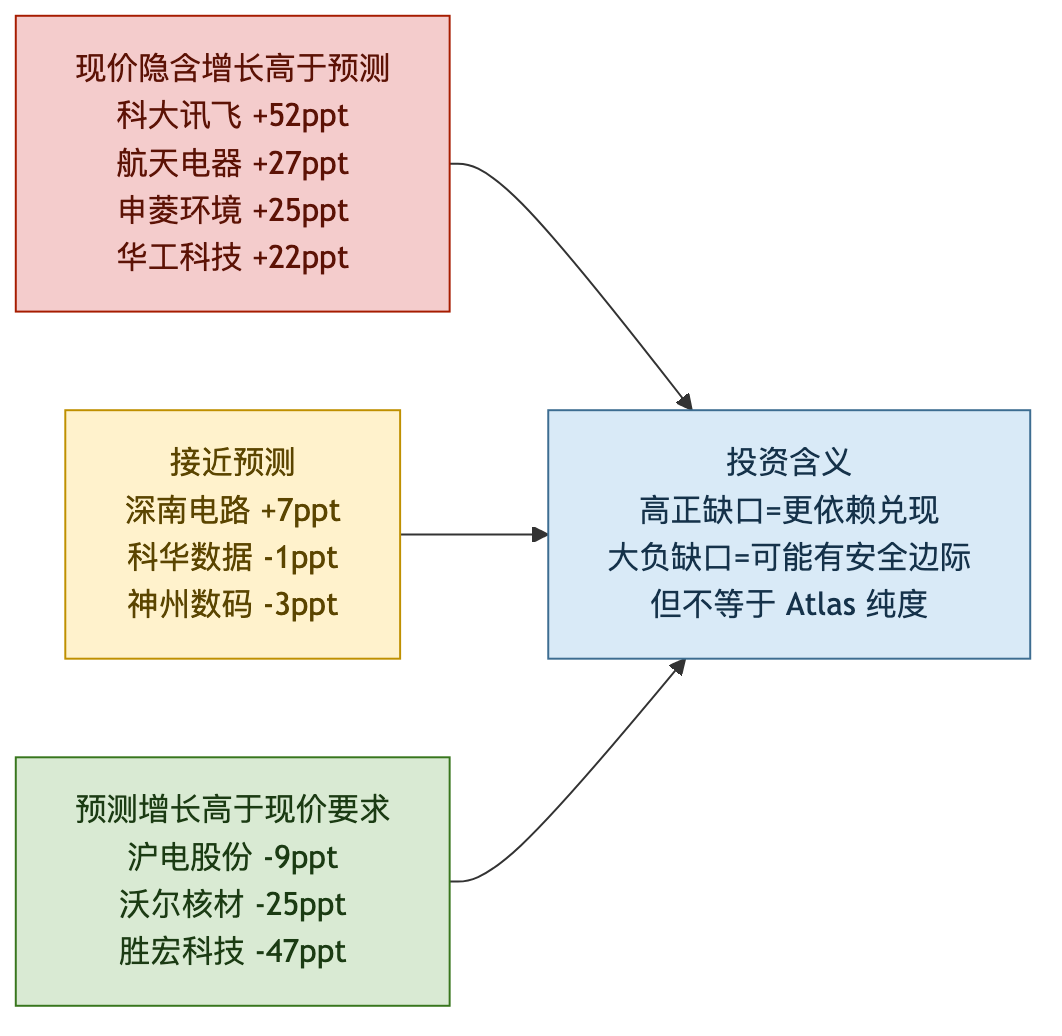
\includegraphics[width=0.96\textwidth]{exhibits/valuation_growth_map.png}
\caption{市场隐含增长与 2027E 盈利预测的逐票分层}
\sourcenote{现价、现股本重算 2026E PE 与原始卖方 2027E 归母净利预测。PEG 仅作零权重预期诊断，不进入目标价。}
\end{figure}

逐票桥显示，科大讯飞、航天电器、申菱环境和华工科技的现价隐含增长显著高于 2027E 预测，价格对兑现更敏感；沃尔核材和胜宏科技的预测增长高于现价诊断要求，但两者 Atlas 关系低，因此潜在安全边际来自原有业务而非华为链纯度。单日大跌与五日成交额只说明拥挤和流动性，不能替代基本面锚。

\begin{keyinsight}[AStock 差异化观点]
市场在定价“架构出现”，本报告只给上市公司定价“可证明的收入和利润”。两者之间的时间差，就是机会来源，也是最大风险来源。
\end{keyinsight}
